\section{Preliminary}\label{sec:preliminary}

\subsection{Training Process of CNN}
Training of neural network is usually done with stochastic gradient descent. The training process consists of two alternate phases: forward phase(FP) and back-propagation(BP). The forward phase randomly select a batch of training inputs and calculates their inference result with the current model. The back-propagation phase calculates the gradient of error to the weights in each layer according to the chain rule. We further separate this phase into weight gradient (WG) phase, which calculates the gradient and update the weights and error back-propagation (EB) phase. An example flow of training a 4 layer network is shown in Figure~\ref{fig:train_prelim}.

\begin{figure}[t]
  \centering
  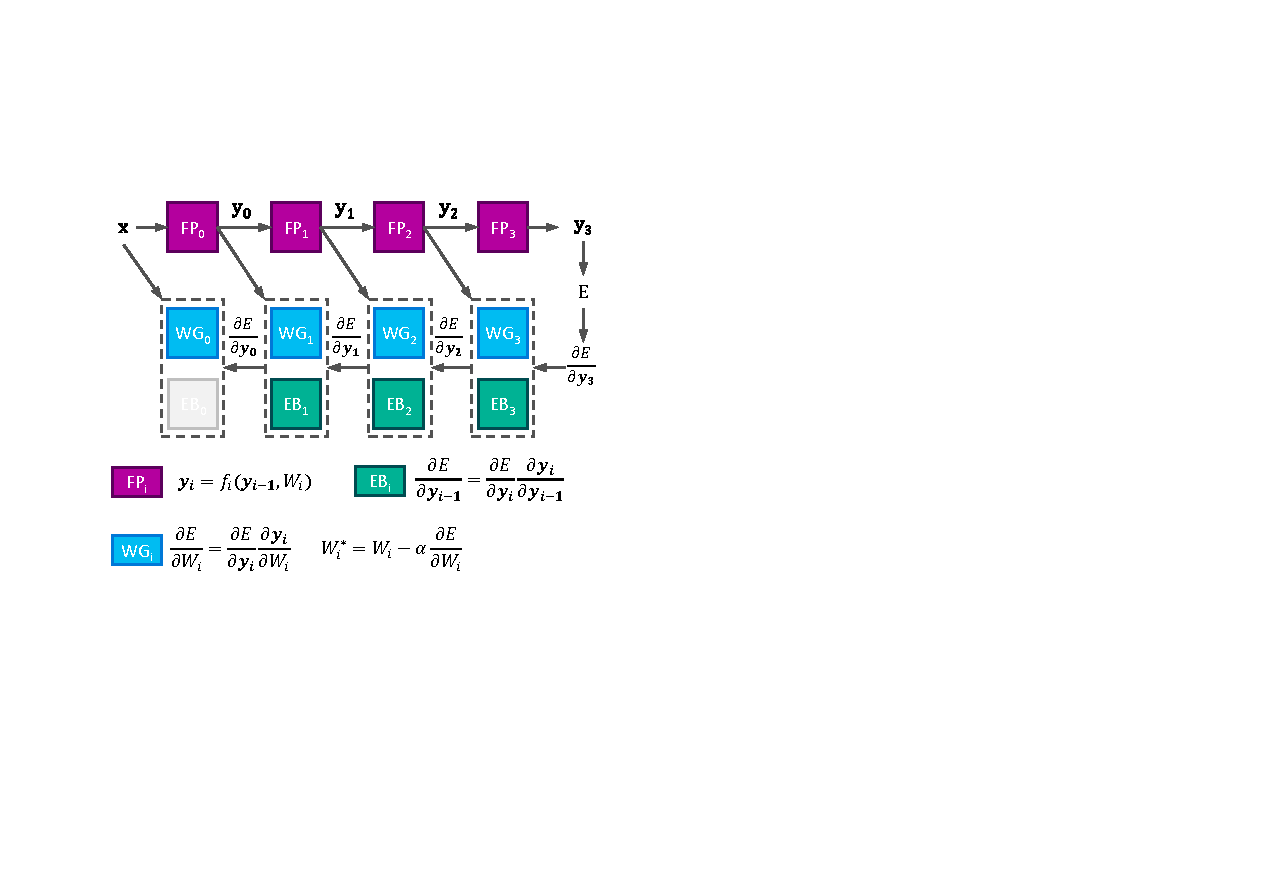
\includegraphics[width=1\columnwidth]{figures/train_prelim.pdf}
  \caption{An example flow of training a 4 layer neural network. }
  \label{fig:train_prelim}
\end{figure}

